% !TeX program = lualatex
% !TeX encoding = utf8
% !TeX spellcheck = uk_UA
% !BIB program = biber
% !TeX root =../QChemBook.tex
\graphicspath{ {\currfiledir/Pictures/} }




%% --------------------------------------------------------
\chapter{Багатоелектронні атоми}
%% --------------------------------------------------------






Опис електронної будови багатоелектронних атомів виявляється істотно складнішим завданням порівняно
із завданням про воднеподібний атом. Річ у тім, що розв'язання квантовомеханічної задачі для атомів з
довільним числом електронів вельми проблематичне і точне аналітичне розв'язання цієї задачі неможливе
для числа електронів, що перевищує $1$. Розв'язання рівняння Шредінгера для багатоелектронного атома
(або молекули) --- предмет галузі науки квантової хімії. Для отримання розв'язку рівняння Шредінгера
або користуються чисельними розрахунками, або розвивають різні наближення.

%Перш ніж обговорювати розв'язання рівняння Шредінгера для довільного багатоелектронного атома,
%розглянемо два відносно простих, але вельми показових випадки: випадок лужних металів і випадок
%атома
%з двома електронами, тобто атома гелію (або в загальнішому сенсі --- гелієподібного атома).






%% --------------------------------------------------------
\section{Атом гелію}
%% --------------------------------------------------------


\begin{wrapstuff}[o, type=figure, 3, width=0.33\linewidth]
	\centering
	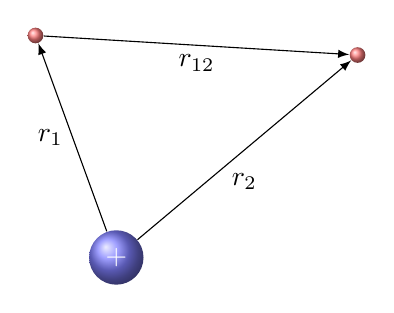
\begin{tikzpicture}[>=latex]
		\node[ball color=blue!50, circle, text=white] (O) at (0,0) {$+$};
		\node[ball color=red!50, circle, inner sep=2pt] (E1) at (110:3) {};
		\node[ball color=red!50, circle, inner sep=2pt]  (E2) at (40:4)  {};

		\draw[->] (O) -- node[left] {$\vect{r}_1$} (E1);
		\draw[->] (O) -- node[below=5pt] {$\vect{r}_2$} (E2);
		\draw[->] (E1) -- node[below] {$\vect{r}_{12}$} (E2);
	\end{tikzpicture}
	\caption{Схематичне зображення атома \ce{He}}
	\label{pic:He}
\end{wrapstuff}
У цьому розділі ми розглянемо випадок атома з двома електронами,
тобто випадок атома гелію. Гамільтоніан атома гелію можна записати в
такому вигляді (рис.~\ref{pic:He}):
\begin{equation}
	\hat{H} = \hat{h}_1 + \hat{h}_2 + \frac1{r_{12}}
\end{equation}
Тут $\hat{h}_1$ і $\hat{h}_2$ --- гамільтоніани кожного з електронів, що взаємодіють із центральним іоном із зарядом $Z = 2$; третій член відповідає
енергії взаємодії електронів один з одним. Обчислимо енергію цієї системи в основному стані.


%% --------------------------------------------------------
\section*{Теорія збурень}
%% --------------------------------------------------------



У нульовому наближенні вважатимемо, що двоелектронна хвильова функція є добутком одноелектронних
хвильових функцій:

\begin{equation}
	\psi_0(\vect{r}_1, \vect{r}_2) = \phi_1(\vect{r}_1)\phi_2(\vect{r}_2).
\end{equation}

Таким чином, поки що ми \emph{нехтуємо впливом одного електрона на хвильову функцію іншого електрона}. Для одноелектронної хвильової функції основного
стану
$\phi(\vect{r})$ запишемо:
\begin{equation*}
	\phi(\vect{r}) = \left( \frac{Z^3}{\pi}\right)^{1/2} e^{-Zr}.
\end{equation*}

Повна енергія в першому порядку теорії збурень дорівнює:

\begin{equation}
E^{(1)} = \langle \psi_0 | \hat{V} | \psi_0 \rangle,
\end{equation}

де:
\begin{itemize}
\item \(\psi_0\) --- хвильова функція основного стану незбуреної системи;
\item \(\hat{V}\) --- оператор збурення, який описує додаткову взаємодію (наприклад,
електрон-електронну взаємодію в атомі гелію).
\end{itemize}

Для атома гелію оператор збурення \(\hat{V}\) має вигляд:
\begin{equation*}
\hat{V} = \frac1{|\mathbf{r}_1 - \mathbf{r}_2|},
\end{equation*}
де \(\mathbf{r}_1\) та \(\mathbf{r}_2\) --- координати першого та другого електронів.

Таким чином, перший порядок поправки до енергії обчислюється як:
\begin{equation*}
E^{(1)} = \int \psi_0^*(\mathbf{r}_1, \mathbf{r}_2) \frac1{|\mathbf{r}_1 - \mathbf{r}_2|}
\psi_0(\mathbf{r}_1, \mathbf{r}_2) \, d\mathbf{r}_1 \, d\mathbf{r}_2.
\end{equation*}

Цей інтеграл можна спростити, використовуючи розклад потенціалу \(\frac{1}{|\mathbf{r}_1 -
\mathbf{r}_2|}\) за сферичними гармоніками або інші методи обчислення кулонівських інтегралів.
Для атома гелію:
\begin{equation*}
    E^{(1)} = \frac58 Z.
\end{equation*}

Ця поправка враховує внесок електрон-електронної взаємодії в енергію основного стану атома гелію.


Енергія атома
\begin{equation*}
    E = E^{(0)} + E^{(1)} = -Z^2 + \frac58Z
\end{equation*}



Підстановка чисельних значень дає такі результати. Якщо врахувати тільки два перших внески, тобто
знехтувати кулонівським відштовхуванням електронів, то енергія дорівнює $- 108.8$~еВ, врахування всіх
трьох внесків дає енергію $-74.8$~еВ, тоді як експериментальне значення енергії дорівнює $-78.9$~еВ.
Очевидно, що нехтування кулонівським відштовхуванням електронів абсолютно не виправдане, однак і
запропонований метод врахування відштовхування не цілком точний --- використання першого порядку
теорії збурень не цілком правомірне, оскільки внески в енергію --- величини одного порядку.


%% --------------------------------------------------------
\section*{Варіаційний метод}
%% --------------------------------------------------------





Щоб «підправити» хвильову функцію, запишемо одноелектронну функцію в наступному вигляді:
\[
\phi(\mathbf{r}, \zeta) = \left( \frac{\zeta^3}{\pi} \right)^{1/2}
e^{-\zeta r},
\]
де \(\zeta\) --- ефективний заряд. Сенс цієї формули полягає в тому, що наявність другого
електрона частково екранує позитивний заряд атомного ядра: як і у випадку лужних металів, кожен
електрон взаємодіє з атомним «остовом», заряд якого дорівнює ефективному заряду \(\zeta\).
Таким чином, крім відштовхування електронів ми враховуємо також вплив електронів на потенціал
притягання до центрального іона. Обчислимо енергію системи при певному значенні \(\zeta\):
\[
E(\zeta) = -2Z\zeta + \zeta^2 + \frac58 \zeta.
\]
%У даному розрахунку внесок від кінетичної енергії для кожного електрона дорівнює
%\[
%\langle \phi(\mathbf{r}_k, \zeta) | \hat{T}_k | \phi(\mathbf{r}_k, \zeta) \rangle =
%\zeta^2 \text{Ry},
%\]
%а внесок від потенціальної енергії взаємодії електрона з ядром ---
%\[
%\langle \phi(\mathbf{r}_k, \zeta) | -\frac{Z e^2}{r_k} | \phi(\mathbf{r}_k, \zeta)
%\rangle = -2Z \zeta \text{Ry}.
%\]
%Нарешті, енергія відштовхування електронів дорівнює
%\[
%\frac{5}{4} \zeta \text{Ry}.
%\]
Далі скористаємося варіаційним принципом квантової механіки.
Для цього визначимо хвильову функцію, яка забезпечує мінімум функціоналу енергії:
\[
\delta \int \psi^* \hat{H} \psi \, d\mathbf{r} = 0
\]
за умови виконання умови нормування: \(\langle \psi | \psi \rangle = 1\). Тут \(\delta\) позначає
варіацію, яку можна проводити як по хвильовій функції \(\psi\), так і по \(\psi^*\), інтегрування
ведеться по всіх просторових координатах \(\mathbf{r}\). При виконанні умови \(\delta \langle \psi |
\hat{H} | \psi \rangle = 0\) ми отримуємо хвильову функцію, максимально близьку до істинної хвильової
функції основного стану. У нашому випадку вигляд пробної хвильової функції задається виразом (2.10),
і, таким чином, застосування варіаційного принципу еквівалентно умові на мінімум функції
\(E(\zeta)\):
\[
\frac{dE(\zeta)}{d\zeta} = 0 \Rightarrow \zeta = Z - \frac{5}{16}.
\]
Підстановка дає наступне значення енергії:
\[
E = -2 \left( Z - \frac{5}{16} \right)^2 .
\]
Чисельне значення цієї енергії \(-77,5\) еВ, що суттєво ближче до експериментального значення. Таким
чином, екранування заряду центрального іона другим електроном дає суттєву поправку до повної енергії.



%% --------------------------------------------------------
\section{Кореляційні ефекти}
%% --------------------------------------------------------


Електрони з повністю заповнених оболонок не беруть участі в утворенні хімічного зв'язку: хімічні
властивості атомів визначаються електронами зовнішньої
оболонки --- \emph{валентними електронами}.


Атоми з одним валентним електроном --- елементи першого періоду в таблиці Менделєєва. Ці елементи (за
винятком водню) --- лужні метали:
\ce{Li}, \ce{Na}, \ce{K}, \ce{Rb}, \ce{Cs}, \ce{Fr}. На перший погляд, розв'язок рівняння Шредінгера
для лужних металів має бути  подібним до розв'язку
для атома водню, тому що електрони внутрішніх оболонок досить компактно розташовані поблизу ядра, а
валентний електрон рухається в сумарному полі
атомного <<остова>>, тобто в полі ядра й електронів із внутрішніх оболонок. У першому порядку
мультипольного розкладання потенціал має вигляд
\begin{equation*}
	U(r) = -\frac{\zeta}{r}
\end{equation*}
де $\zeta$ --- ефективний заряд остова ефективний заряд остова. Однак слід врахувати, що валентний
електрон збурює, а саме, поляризує атомний остов,
наводячи на ньому ефективний дипольний момент. У результаті ефективний потенціал взаємодії з остовом
змінюється, а співвідношення $U(r) \sim  -\frac1r$
порушується. Таким чином, потенціал спотворюється і відрізняється від кулонівського.


\begin{wrapstuff}[type=figure, l, width=0.33\linewidth]
	\centering
	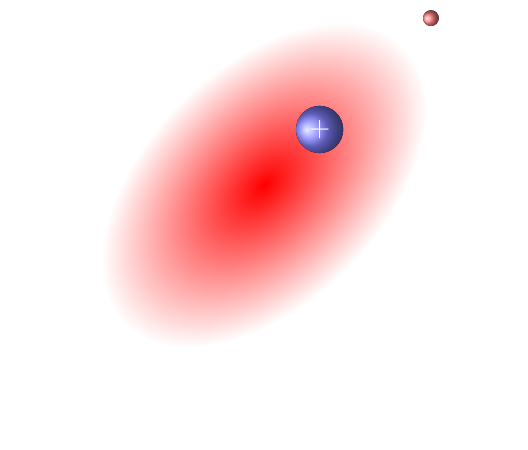
\begin{tikzpicture}
		\begin{scope}[transform canvas={rotate=45}]
			\path[inner color=red, outer color=white] (0,0) circle(2.5 and 1.5);
			\fill[ball color=blue!50] (+1,0) circle (0.3) node[text=white, font=\bfseries,
					rotate=-45] {$+$};
			\fill[ball color=red!50]  (0:3) coordinate (E2) circle (0.1);
		\end{scope}
		\path (-3, -3) rectangle (3,2);
	\end{tikzpicture}
	\caption{Поляризація остова}
\end{wrapstuff}
Слід очікувати, що в результаті буде знято <<випадкове>> виродження
за орбітальним моментом. Дійсно, уявімо потенціал у вигляді:
\begin{equation}
	U(r) = -\frac{\zeta e^2}{r} + C_1\frac{\zeta e^2}{r^2},
\end{equation}
де $C_1$ -- константа, що характеризує величину наведеного дипольного моменту. Як правило, $\zeta$
обчислюють за простою формулою $\zeta = Z - N$
(де $N$ --- число електронів остова), хоча існують і складніші варіанти апроксимації потенціалу
остова. Звернемо увагу на те, що функціональна
залежність від відстані для потенціалу $ C_1\frac{\zeta e^2}{r^2} $ збігається з такою для
відцентрового потенціалу $ \frac{\hbar}{2m_e}\frac{l(l +
		1)}{r^2}$ .
Тому появу додаткового внеску в $U(r)$ можна представити як перевизначення квантового числа $l$:
\begin{equation*}
	\frac{\hbar}{2m_e}\frac{l(l + 1)}{r^2} + C_1\frac{\zeta e^2}{r^2} =
	\frac{\hbar}{2m_e}\frac{l^*(l^* + 1)}{r^2}.
\end{equation*}

Звідки отримуємо за малих$C_1$
\begin{equation}
	l^* = l - \frac{m_e\zeta e^4}{\hbar \left( l + \frac12 \right) }.
\end{equation}
Далі, візьмемо до уваги, що головне квантове число дорівнює ($n = n_r + l + 1$), де $n_r$ ---
радіальне квантове число, що виникає при
поділу змінних у рівнянні Шредінґера. Будемо вважати, що при появі дипольної добавки до потенціалу
число $n_r$ не змінюється, тоді як $l$ замінюється на
$l^*$. Тоді головне квантове число змінюється таким чином:
\begin{equation*}
	n \to n^* = n_r + l^* + 1 = n - C_1 \frac{m_e\zeta e^4}{\hbar \left( l + \frac12 \right) } = n
	- \Delta_l.
\end{equation*}

\begin{wrapstuff}[type=table, l, 5, width=0.33\linewidth]
	\caption{Дефект для основного терму лужних металів}\label{tab:Defect}
	\centering
	\begin{tblr}{
		colspec={X[l,m]Q[c,m]Q[c,m]},
		column{1} = {mode=math},
		column{2} = {mode=math},
		column{3} = {mode=math},
		}
		\toprule
		\text{Элемент} & n & \Delta_l \\
		\midrule
		\ce{Li}        & 2 & 0.41     \\
		\ce{Na}        & 3 & 1.37     \\
		\ce{K}         & 4 & 2.23     \\
		\ce{Rb}        & 5 & 3.20     \\
		\ce{Cs}        & 6 & 4.13     \\
		\bottomrule
	\end{tblr}
\end{wrapstuff}
Для розрахунку енергії скористаємося формулою для водородоподібного атома:
\begin{equation}
	E = - \Ry \frac{\zeta}{n^{*2}} = - \Ry \frac{\zeta}{(n^2 - \Delta_l)}.
\end{equation}
Величина $\Delta_l$  називається квантовим дефектом, ця поправка призводить, як і очікувалося, до
зняття виродження за орбітальним моментом. Зазначимо,
що зі зростанням $l$ ця поправка зменшується, оскільки ймовірність знаходження валентного електрона
поблизу атомного остова
швидко зменшується, тобто $C_1$, і $\Delta_l$ істотно зменшуються за величиною. Збуджені атоми лужних
металів, у яких валентний електрон перебуває в
стані з більшими $n$ і $l$, називають \emph{рідбергівськими атомами}. У рідбергівських атомах з
хорошою точністю працюють формули для воднеподібних
атомів.

Зазначимо, що при $\Delta_l \neq 0$ енергія знижується порівняно з величиною $E =
-\Ry\frac{Z^2}{n^2}$, оскільки положення валентного електрона через
закони квантової механіки розподілене в просторі і валентний електрон деякою мірою <<проникає>>
всередину деякою остова. Величини квантових
дефектів для низки випадків наведено в табл.~\ref{tab:Defect}.

